\documentclass{standalone}

\usepackage{amssymb}
\usepackage{tikz}
\usetikzlibrary{calc}

\begin{document}
  %noformat{
  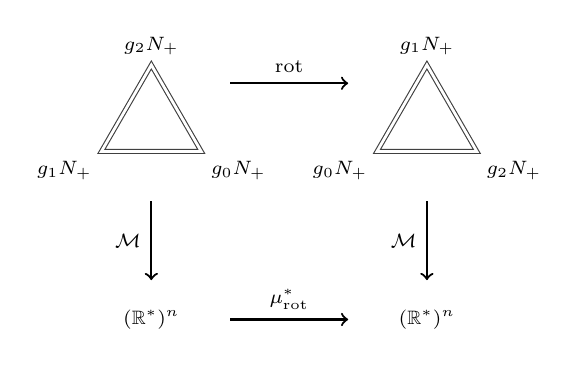
\begin{tikzpicture}
    \tikzstyle{te} = [color=darkgray, double distance=1pt]

    \tikzset{font=\scriptsize}

    \begin{scope}[shift={(0.0,0)}]
      \coordinate[label={330:$g_0 N_{+}$}] (l_0) at (-30:0.7321);
      \coordinate[label={210:$g_1 N_{+}$}] (l_1) at (210:0.7321);
      \coordinate[label={ 90:$g_2 N_{+}$}] (l_2) at ( 90:0.7321);

      \draw[te] (l_0) -- (l_1) -- (l_2) -- cycle;
    \end{scope}

    \begin{scope}[shift={(3.5,0)}]
      \coordinate[label={210:$g_0 N_{+}$}] (l_0) at (210:0.7321);
      \coordinate[label={ 90:$g_1 N_{+}$}] (l_1) at ( 90:0.7321);
      \coordinate[label={330:$g_2 N_{+}$}] (l_2) at (-30:0.7321);

      \draw[te] (l_0) -- (l_1) -- (l_2) -- cycle;
    \end{scope}

    \node (c1) at (0.0, -2.5) {$(\mathbb{R}^{\ast})^n$};
    \node (c2) at (3.5, -2.5) {$(\mathbb{R}^{\ast})^n$};

    \draw[->, thick]
        (1.0,0.5)
        to[] node[midway, above] (t04) {$\mathrm{rot}$}
        (2.5,0.5);
    \draw[->, thick]
        (0.0,-1.0)
        tonode[midway, left] (t01) {$\mathcal{M}$}
        (0.0,-2.0);
    \draw[->, thick]
        (3.5,-1.0)
        tonode[midway, left] (t02) {$\mathcal{M}$}
        (3.5,-2.0);
    \draw[->, thick]
        (1.0,-2.5)
        to[] node[midway, above] (t03) {$\mu_{\mathrm{rot}}^{\ast}$}
        (2.5,-2.5);
  \end{tikzpicture}
  %}noformat
\end{document}
